\section{Backend}
\label{desenvolupament:backend}
Al llarg d'aquesta secció, farem referència a l'evolució al llarg del temps de la part servidora del projecte, encarregada de la gestió de les dades, així com de la comunicació amb serveis externs.\\
\newline Per tant, el \textit{backend} serà l'encarregat de la gestió de tot el procés d'emissió, signatura i validació de consentiments informats, enviar les dades al \textit{frontend}, rebre'n de noves, i actualitzar les existents en cas de ser necessari.\\
\newline Per tant, el que s'espera del \textit{backend} és el següent:
\begin{itemize}
    \item Generació i emissió de documents (consentiments informats)
    \item Gestió de la signatura electrònica de documents
    \item Validació de documents
\end{itemize}
\clearpage
\subsection{Model inicial}
La idea inicial per al \textit{backend} és fer servir aquest tercer de confiança (Secció \ref{estatArt:thirdparty}) per tota la gestió de certificació i signatura de documents.\\
\newline El tercer de confiança escollit per a l'ocasió, \textit{Lleida.net}, ofereix serveis de signatura electrònica mitjançant OTP (Secció \ref{arquitectura:otp}), certificació de documents i en cas de necessitar-ho, mecanismes per assegurar el no repudi dels documents signats.\\
\newline Així doncs, en vistes dels serveis que ofereix \textit{Lleida.net}, el sistema a implementar ha d'actuar de pont entre la plataforma \textit{MoG} i els serveis del tercer de confiança.\\
\newline Per tal d'il·lustrar el funcionament, la figura \ref{fig:thirdparty_usage} mostra un esquema de les interaccions entre el tercer de confiança i el mòdul desenvolupat per aquest TFG:
\begin{figure}[h]
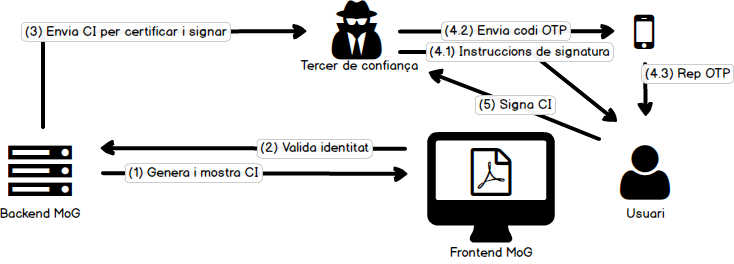
\includegraphics[scale=0.55]{sections/developement/trusted_thirdparty_arch.png}
\centering
\caption{Ús de tercers de confiança}
\label{fig:thirdparty_usage}
\end{figure}
\newline Veient la figura superior, ens n'adonem que les accions de pes recauen íntegrament sobre les espatlles del tercer de confiança, quedant per al projecte que aquí es desenvolupa les funcions d'interlocutor entre \textit{Lleida.net} i el \textit{backend}, i generar els consentiments informats.
\subsubsection{Generació de consentiments informats}
\begin{listing}[h]
\inputminted[
    firstline=74, 
    lastline=83,
    fontsize=\footnotesize]{php}{resources/src/InformedConsentGeneratorService.php}
\caption{Crida a la funció de renderitzat de Twig}
\label{code:twigRender}
\end{listing}
El fragment de codi anterior, mostra una crida a la llibreria de renderitzat de \textit{Symfony}\footnote{https://symfony.com/}. Juntament amb la llibreria \textit{wkhtmltopdf}\footnote{https://wkhtmltopdf.org/} es fan servir per, primerament, incrustar contingut dinàmicament a una plantilla HTML\footnote{HyperText Markup Language} i després, transformar aquest HTML en pdf mantenint els CSS\footnote{Cascading Style Sheets} de la plantilla.
\subsubsection{Funcionament del tercer de confiança i repercusions}
Tot i ser una dinàmica pròpia del tercer de confiança, és important conèixer el funcionament del servei que s'està a punt de fer servir.\\
\newline Com es pot veure a la Figura \ref{fig:thirdparty_usage}, el procés de certificació i posterior signatura segueixen una sèrie de passos estructurats i ben definits.
Un cop l'usuari ha validat la seva identitat, el \textit{backend} llança l'ordre de signatura del document que s'acaba de crear. Per això, s'envia un correu al tercer de confiança amb el document que es vol certificar i el destinatari (signant).\\
\newline Per la seva banda, \textit{Lleida.net}, en rebre l'ordre envia un segon correu a l'usuari amb:
\begin{itemize}
    \item Consentiment informat certificat.
    \item Instruccions per a la signatura.
    \item Enllaç a la web per signar el document.
\end{itemize}
Un cop l'usuari ha signat el document, \textit{Lleida.net} informa a l'emissor que la signatura del document s'ha dut a terme correctament.\\
\newline En aquest punt, on sembla ser que tot el procés s'ha dut a terme satisfactòriament, apareix el primer contratemps d'aquest projecte, i que provocarà un canvi d'estratègia global.\\
\newline \textit{Lleida.net} posa a disposició de l'emissor del document una plataforma des d'on recuperar els documents certificats.\\
\newline La impossibilitat d'automatitzar el procés obliga a recuperar de forma manual els documents, fet inadmissible ja que en termes d'escalabilitat, en el moment en que s'hagin de signar centenars de consentiments informats, amb la seva corresponent recuperació, el temps i l'esforç requerit seran massa grans.\\
Per tant, aquest fet obliga a descartar aquesta idea inicial.%ja que en el supòsit de que s'hagin de recuperar centenars de documents, com ja s'ha dit, s'hauria de fer manualment.

%\newline Com es pot veure, tota la activitat depèn íntegrament d'aquesta entitat externa. Un cop l'usuari ha validat la seva identitat com a signant, s'informa al tercer de confiança que ha d'iniciar el procés de signatura del document adjunt a l'ordre.\\
%\newline Aquest procés culmina amb un correu electrònic per part del tercer de confiança a l'usuari, on s'adjunta el consentiment informat certificat, unes instruccions a seguir per a signar el document i l'enllaç per a signar-lo.\\
%\newline La part fosca, i la que posa fi a la idea de fer ús dels serveis del tercer de confiança, és la manca d'una forma que es pugui automatitzar la recuperació dels documents certificats i signats. El tercer de confiança posa a disposició del seu client una plataforma que permet recuperar els resultats de les operacions que hagi dut a terme.
\clearpage
%Entesos el model de negoci de l'empresa i les necessitats a les quals es busca donar solució a través d'aquest Treball de Final de Grau, era necessari desenvolupar un projecte el més complet i funcional possible per tal de integrar-lo posteriorment amb la plataforma \textit{Made of Genes}.\\
%A partir de les dades proporcionades i dels diferents casos d'ús i escenaris a contemplar, es comença a dissenyar un primer esquema de model de dades i de funcionalitats.\\
%\newline Al llarg dels apartats d'aquesta secció veurem com va anar evolucionant, i quines decisions es van prendre en relació al \textit{backend} al llarg del transcurs i del desenvolupament d'aquest projecte.\\
%\newline A més, a mesura que s'avanci en l'explicació, es presentaran tant conceptes com noves parts que vagin apareixent al llarg del projecte.
%\subsection{Passos i idees inicials}
%Inicialment, tal i com s'ha esmentat diverses vegades al llarg del document, el projecte basa el seu "nucli"  amb eines oferides per unes entitats anomenades tercers de confiança.\\
%La idea inicial del projecte es la d'usar els serveis que ofereixen aquestes entitats, per tal d'externalitzar la signatura dels documents.\\
%\newline L'arquitectura resultant d'aquest objectiu esdevé en el següent esquema:\\
%\newline \textbf{\textit{Imatge esquema tercer de confiança}}\\
%\newline Com es pot veure a la imatge superior, la plataforma genera un document \textit{.pdf} corresponent a un consentiment informat, fruit de la compra d'un servei per part del pacient, o en el seu defecte la prescripció d'un servei a un pacient per part d'un  metge; aquest document es mostra al pacient a través del frontend (posteriorment la plataforma \textit{Made of Genes}). Per una altra banda, també s'enviarà al pacient a través del tercer de confiança el qual, prèviament, haurà signat, amb un certificat propi, aquest document per tal d'assegurar-ne l'autenticitat i el contingut i re-enviarà al pacient.\\
%El pacient rebrà el document i, en cas d'estar conforme amb tot el que s'hi explica, el signarà electrònicament fent ús d'un servei d'OTP que ofereix el mateix tercer de confiança.
%\\Un cop el pacient ha signat el consentiment informat, el tercer de confiança desa el consentiment signat, i en gestiona les proves de verificació en cas de ser necessàries.\\
%\newline Amb aquest full de ruta, el desenvolupament del projecte passa a ser un projecte que busca integrar un servei ofert per una companyia externa, tercer de confiança, que satisfà inicialment totes les necessitats plantejades i que suposa una càrrega de treball reduïda.\\
%\newline Pel que fa al model de dades, els canvis a realitzar dins del model actual de base de dades, és mínim.\\
%\newline \textit{\textbf{parlar sobre el model de dades}}\\
%\newline Per la seva simplicitat i les eines que oferia per facilitat la integració, es va triar \textit{Lleida.net} com a opció més viable.\\
%\textit{Lleida.net} disposa d'un seguit de llibreries en diferents llenguatges que permeten una fàcil integració del seu servei amb la plataforma, així com la possibilitat d'iniciar el flux de certificació de consentiment informats i posterior signatura per part del client, enviant un correu electrònic a una determinada compte de correu amb un assumpte pre establert.\\
%\newline El problema surt a la llum durant l'última fase del procés d'integració del mòdul desenvolupat amb el servei de \textit{Lleida.net}, quan per poder accedir al document signat, és necessari accedir-hi a través d'una plataforma pròpia del tercer de confiança; provocant així un canvi de context molt fort, i totalment inadmissible dins d'una plataforma que el que busca precisament és la unificació i homogeneïtzació dels seus serveis.\\
%\newline Aquest canvi de rumb obliga a buscar solucions que permetin satisfer les necessitats existents amb el grau de personalització desitjat, fins i tot si aquestes possibles solucions impliquen abandonar el concepte del tercer de confiança en espera d'una solució que s'ajusti més al desitjat en un primer moment.\\
%En aquesta ocasió, vistes les alternatives pel que fa a tercers de confiança i les seves possibles solucions, la possibilitat d'un canvi de tecnologia semblava d'allò més plausible.\\
%Arribats a aquest punt del desenvolupament, conceptes com \textit{Blockchain}, %\textit{OTP} i \textit{empremta digital} prenen força dins del projecte.\\
%\newline Per una banda cal substituir totes les funcionalitats que fins ara depenien íntegrament del tercer de confiança:
%\begin{itemize}
%    \item Validació del contingut del document
%    \item Signatura del document
%    \item Assegurar el no repudi 
%\end{itemize}
%I per l'altra banda dotar al nou procés de la validesa i robustesa legal necessària.\\
%La primera idea que ve al cap és la d'adquirir un certificat propi expedit per a una Autoritat Certificadora (CA) reconeguda i fer els canvis pertinents dins de la plataforma per tal de que poder treballar amb el certificat digital. El problema d'aquesta idea és que se surt del pressupost est
\subsection{Cerca d'alternatives}
\label{desenvolupament:alternatives}
En vistes del succeït, el no poder acabar la integració del tercer de confiança amb el \textit{backend} de l'aplicació, suposa un canvi de rumb molt important, per no mencionar l'endarreriment del projecte, que provoca l'inici d'un procés de recerca d'alternatives viables per a poder continuar.\\
\newline Després d'un procés de recerca i valoració, els candidats finals són tres:
\begin{itemize}
    \item Buscar un tercer de confiança alternatiu.
    \item Adquirir un certificat reconegut.
    \item Sistemes de \textit{timestamping} distribuïts (\textit{blockchain}).
\end{itemize}
La tendència és la de buscar un tercer de confiança alternatiu que s'adapti a les necessitats del projecte. Malauradament, el gruix d'entitats alternatives, tenen un funcionament similar al de la primera i la resta ofereixen llibreries on l'esforç necessari per a una bona integració és massa elevat i requereix massa temps, temps del que no es disposa.
\newline Un cop eliminada la primera opció, manquen les opcions que tenen a veure amb la implementació total d'un sistema que permeti emetre, signar i validat consentiments informats.\\
\newline Tal i com es diu a la secció \ref{estatArt:signature} d'aquest mateix document, l'ús d'un determinat sistema de signatura electrònica queda reconegut davant la llei sempre i quan les dues parts interessades hi estiguin d'acord.\\ La plataforma principal ja disposa d'un sistema d'SMS funcional. Per tant sols manca el desenvolupament del servei capaç de crear/validar codis OTP i decidir la millor forma de certificar el contingut dels documents generats.\\
\newline La primera de les alternatives a tenir en compte és l'adquisició d'un certificat digital emès per una CA\footnote{Certification Authority} reconeguda que permeti a \textit{Made of Genes} la certificació dels seus propis documents.\\
\newline El principal inconvenient d'aquesta segona opció és la necessitat de renovar cada cert temps el certificat.\\
%No obstant, de moment es postula com la opció que més s'adapta a les necessitats del projecte.\\
\newline La tercera opció que es planteja, és la de fer ús de les capacitats ``tamper-proof'' de la \textit{blockchain} (descrita amb més detall a la secció \ref{estatArt:blockchain}) per tal de certificar el contingut dels documents que s'han signat.\\
\newline Aquesta opció, a primera vista no té cap mena d'inconvenient, donat que es una alternativa de cost zero i que existeixen serveis que permeten l'accés a la \textit{blockchain} d'una forma senzilla i ràpida.\\
\newline Després de valorar les alternatives, s'ha decidit posar en pràctica la tercera via.

%En front del fracàs i conseqüent endarreriment en el projecte que suposa el no poder culminar la integració amb el tercer de confiança, cal començar un procé de selecció per a trobar un nou full de ruta dins del desenvolupament del projecte.\\
%\newline Els tercers de confiança alternatius, o bé ofereixen un servei similar al que ja ha quedat descartat o la llibreria que ofereixen per a integrar el seu servei no s'ajusta al que es busca o bé necessita una quantitat de feina desmesurada, i que impossibilitaria l'execució del TFG a temps.\\
%\newline Un cop eliminada la possibilitat d'externalitzar la certificació i signatura dels consentiments de documents, cal trobar la forma de suplir aquestes dos tasques.\\
%Per la part que correspon a la signatura del document, sempre que la llei ho permeti es vol continuar utilitzant el concepte de codi OTP i signatura digital.\\
%Tal i com es diu a la secció \ref{estatArt:signature} d'aquest mateix document, l'ús d'un determinat sistema de signatura electrònica queda reconegut davant la llei sempre i quan les dues parts interessades hi estiguin d'acord.\\
%Per tant, queda coberta la part de signatura. Manca trobar una solució per la part de certificació de documents.
%\newline La segona alternativa a contemplar en referència a assegurar el contingut dels documents, passa per l'obtenció d'un certificat digital reconegut.\\
%\newline Fer ús d'un certificat digital emès per una CA\footnote{Certification Authority} reconeguda implica la total autonomia a l'hora de legitimar el contingut dels consentiments emesos per la plataforma.\\
%\newline Per contra el temps que es necessita per implantar i implememtar aquesta solució és major del que es busca. Addicionalment, un certificat s'ha de renovar cada cert temps, fet que suma punts en contra.\\
%\newline La tercera i última alternativa, consisteix en fer ús de tecnologies descentralitzades, com es el cas de \textit{blockchain} (Secció \ref{estatArt:blockchain}) que permeten el fer segellat de temps d'informació d'una forma a prova de modificacions.\\
%\newline Aquesta tercera opció, és la que després de valorar les alternatives, és la que s'ha acabat implementant al TFG.

%La primera reacció al ser conscients del fracàs i el conseqüent endarreriment que suposa el no poder finalitzar la integració amb \textit{Lleida.net}, és la de buscar una alternativa a aquest que permeti continuar "externalitzant" la part de certificació i signatura de documents.\\
%El resultat és una llista de tercers de confiança que, o bé per l'ús d'una plataforma similar per a la gestió de documents, o bé per que les eines que ofereixen no solucionen el problema, o bé per que el cost d'integració fent ús de les seves eines suposa un problema major, la idea de fer ús d'un tercer de confiança com a entitat certificadora i de validació de documents queda totalment descartada.\\
%\newline La següent opció a tenir en compte, es basa en l'obtenció d'un certificat pròpi emés per una Autoritat Certificadora (CA) reconeguda, modificar el mòdul per certificar els documents emesos pel mateix i fer ús d'un sistema d'OTP pròpi.\\
%Aquest, és un procés costós i que requereix implementar tota la infraestructura necessària per a la certificació i posterior val·lidació.\\
%Per aquests motius, és una línia que es decideix abandonar en post d'idees un xic més innovadores però sempre tenint-la en compte per si en algun moment s'ha de tornar a quest model.\\
%\newline Finalment, la tercera alternativa es basa en l'ús d'una tecnologia emergent anomenada \textit{Blockchain}, popularitzada per ser la tecnologia en la que la moneda virtual \textit{Bitcoin} basa el seu funcionament.\\
%Aquesta última opció, és la que per les raons que s'exposaran a continuació ha acabat sent implementada al projecte.\\
%\newline \textit{Made of Genes}, com s'ha dit diverses vegades al llarg del document, és una \textit{startup}, altrament dit empresa jove, amb recursos limitats i que no es poden malbaratar. Per aquest motiu, un dels factors determinants en l'execució dels diferents projectes i la presa de decisions, és el cost que tindran aquests per l'empresa.\\
%Partint de l'anterior argument, un factor decisiu en la tria de solucions és que suposarà ja no només en temps, si no també en recursos, humans i econòmics.\\
%La plataforma \textit{Made of Genes} ja disposa d'un sistema d'enviament d'SMS que es re-aporfitarà per a l'enviament de còdis OTP per a la signatura.\\
%\newline Manca doncs, un sistema que ens permeti validar d'alguna forma el contingut dels documents i assegurar-ne el no repudi en cas de conflictes, en aquest punt es on entra en joc \textit{Blockchain}.\\
%\newline En capítols anteriors d'aquest document, s'exposa el funcionament i estructura de \textit{blockchain} de forma més extensa.
%\subsection{Canvis en el projecte}
%Un cop segurs del nou rumb a seguir, cal valorar els canvis necessaris per adoptar la nova metodologia de funcionament que seguirà el \textit{backend} del projecte.\\
%Els canvis es poden agrupar en dos grups:
%\begin{enumerate}
%    \item Aquells que fan referència a la signatura de consentiments informats.
%    \item Aquells que fan referència a la validació i a assegurar el no repudi de documents.
%\end{enumerate}


%Fins l'abandonament dels serveis oferts pel tercer de confiança, els documents es signaven mitjançant l'enviament, per part d'aquest tercer, de missatges SMS amb un codi únic (o OTP) generat per a l'ocasió; la idea és dotar a la plataforma de la capacitat de generar aquests codis OTP, d'enviar-los i validar-los.
%Per a l'enviament, es farà ús del servei ofert per \textit{Clickatell}, un servei que ja es fa servir en altres processos dins de la plaforma \textit{Made of Genes} i que té un cost per missatge molt reduït.\\
%\newline \textit{Clickatell} ofereix una llibreria en format de \textit{bundle} pensada per integrar amb projectes basats en \textit{Symfony}, framework PHP sobre el que es construeix el \textit{backend} on, el que manca per fer, seguint el principi de desenvolupament S.O.L.I.D, és desenvolupar un servei al voltant de la llibreria que ens permeti independitzar-la del nostre codi; d'aquesta manera aconseguim que si en algun moment apareix una alternativa a \textit{Clickatell} que pel motiu que sigui interessa més, sigui fàcilment substituïble.\\
%Per a la generació del còdi OTP, farem ús de l'algorisme definit al RFC6238 (TOTP: Time-Based One-Time Password Algorithm) i la variació d'aquest últim definida a l'RFC4226 (HOTP: An HMAC-Based One-Time Password Algorithm).\\
%\newline \textbf{\textit{Parlar una mica del que diuen els RFC.... P-A-L-A-Z-O}}\\
%\newline Pel que fa a la validació del contingut dels documents i assegurar el seu posterior no repudi, com ja es va anticipant unes línies enrere, es vol fer servir \textit{Blockchain}.\\
%La tecnologia de \textit{blockchain} s'explica amb detall al capítol 3 del document.\\
%\newline Aplicada concretament al projecte que ens ocupa, es busca aprofitar el funcionamet i la potència de \textit{blockchain} per assegurar el no repudi dels documents mitjançant la publicació de l'empremta digital (hash SHA-256) del consentiment informat via petites transaccions de bitcoin.\\
%Per fer una mica de memòria, el hash d'un document, com s'ha explicat en capítols anteriors del document, és una cadena de caràcters generada partir del contingut del mateix document.\\
%Unint el hash generat del document a la \textit{blockchain}, s'assegura que el contingut del document que s'acaba de signar, queda registrat on ningú el podrà modificar sense que algú altre se n'adoni; recordem que un cop un bloc actualitza les seves transaccions i les replica a 6 blocs diferents, el contingut d'aquest blocs, i en conseqüencia les transacions registrades, és inmutable.\\
%Per a dur a terme aquesta tasca, s'ha buscat un servei que ens permeti publicar les empremtes digitals dels documents genetrats a la \textit{blockchain}; el servei es qüestió es l'anomenat \textit{Origin Stamp}.\\
%\textit{Origin Stamp} és un servei sense ànim de lucre que facilita la publicació de hashos a la \textit{blockchain} a través de micro transaccions de satoshis, la unitat més petita de bitcoin, equivalen a 0.00000001 bitcoins.\\
%El funcionament del servei és senzill; \textit{Origin Stamp} agrega hashs durant 24 hores a través d'una senzilla API Rest o des del propi portal del servei, que permet pujar fitxers i calcular-ne l'emprempta digital o bé introduïr el propi hash prèviament calculat per l'usuari; un cop superat aquest lapse de 24 hores, realitzen una transacció bitcoin equivalent a un satoshi.\\
%El contingut d'aquesta transació, és un hash que agrega tots els hash acumulats al llarg d'aquestes 24 hores.\\
%En cas de que es desitgi la immediata publicació a la blockchain, el servei accepta donacions d'1\$.
\clearpage
%\subsection{Fase final}
%La recta final del desenvolupament del backend del projecte, s'inicia en el moment en el que s'acaba l'adaptació del mateix amb les noves metodologíes de funcionament.\\ 
%Un cop arribats a aquest estadi, es decideix que el que s'ha de publicar a la \textit{blockchain} no és el hash del consentiment informat, sino el hash d'un document que certifiqui que un usuari determinat, en un moment determinat i amb un codi OTP determinat, ha signat mitjançant l'anterior OTP un consentiment informat amb una empremta digitar determinada.\\
%Per aquest fet, es decidieix modificar la forma amb la que es generen els documents; creant un microservei encarregat d'aquesta tasca.\\
%Aquest nou microservei disposa d'una senzilla API Rest que ens permet enviar les dades necessàries per a que ens torni com a resposta el contingut, codificat en base64, del document desitjat; ja sigui el consentiment informat o bé el coprovant de signatura.\\
%Amb la creació d'aquest microservei independitzem el procés de creació de documents del nucli del projecte, alhora que guanyem una important millora en el temps de creació de documents.\\
%\newline L'esquema resultant del projecte és el següent:\\
%\newline \textit{\textbf{esquema resultant de la plataforma}}\\
%\newline \textit{\textbf{Parlar dels canvis al model de dades + esquema de les taules}}
%Pel que fa al model de dades resultant, hem passat d'un simple parell de taules a la base de dades (figura anterior), a tenir-ne unes cuantes més, a la figura següent es pot veure el model resultant:\\
%\newline \textbf{\textit{model actual}}
\subsection{Model final}
Una vegada decidit el nou rumb que segueix el desenvolupament, cal tenir clares quines son les tasques que manca desenvolupar:
\begin{itemize}
    \item Generar i validar OTP.
    \item Certificar signatura i contingut del consentiment informat.
\end{itemize}
Cal recordar que la capacitat d'enviar SMS ja està integrada dins de la plataforma \textit{Made of Genes}, per tant es pot reutilitzar sense problemes.
\subsubsection{Generació i validació d'OTPs}
Per a la generació de codis OTP (secció \ref{estatArt:signature}), s'ha implementat fil per randa l'algorisme descrit al quart punt de l'especificació\footnote{https://tools.ietf.org/html/rfc6238#section-4}.\\
\newline Seguint amb les directrius de codi que donen la \nameref{arquitectura:back_clean} i \nameref{arquitectura:back_solid}, s'ha encapsulat el codi i modularitzat de tal forma que sigui senzill de llegir i mantenir.
%\begin{itemize}
%\item El primer ragment fa referència a la creació de codis OTP
\begin{listing}[h]
\inputminted[
    firstline=120, 
    lastline=131,
    fontsize=\footnotesize]{php}{resources/src/OTPService.php}
\caption{Mètode de creació de codis OTP}
\label{code:createOTP}
\end{listing}
%\item El segon fragment, a la validació.
\begin{listing}[h]
\inputminted[
    firstline=299, 
    lastline=315,
    fontsize=\footnotesize]{php}{resources/src/OTPService.php}
\caption{Mètode de validació de codis OTP}
\label{code:validateOTP}
\end{listing}
%\end{itemize}
\newline Els fragments de codi que es poden veure sobre aquestes línies, representen cada un dels casos d'ús vistos a la secció \ref{arquitectura:otp} en referència la generació i validació de codis OTP, respectivament.\\
\newline Si es mira el codi detingudament, es pot apreciar que ambdós mètodes tenen pràcticament el mateix comportament, idèntiques crides a funcions.\\
\newline La diferència es troba en el fragment que correspon al procés de validació (Fragment \ref{code:validateOTP}). Aquest executa \textit{n} vegades el procés de generació de codis OTP, sent \textit{n} un enter que oscil·la entre \textit{-TIME\_RANGE} i \textit{TIME\_RANGE}, sent \textit{TIME\_RANGE} una constant definida al codi que actua com a finestra de temps, que permet donar un temps de validesa al codi OTP.\\
\newline Si el codi generat a cada iteració és igual que el codi que s'està evaluant, s'atura l'exeució i el sistema retornarà \textit{true}. En cas contrari, \textit{false}.\\
\newline Els mètodes \textit{oath\_hotp} i \textit{oath\_truncate} es poden trobar a l'annex titulat ``\nameref{appendix:otp}''.

\subsubsection{Certificació de signatura del consentiment informat}
Com s'ha dit a la secció anterior d'aquest mateix capítol (\nameref{desenvolupament:alternatives}), per a la certificació de signatures es farà ús de \textit{blockchain}.\\
Per a una descripció detallada sobre aquesta tecnologia, veure la secció \ref{estatArt:blockchain}.\\
\newline L'objectiu d'aquest punt, és poder donar proves irrefutables de que en un moment donat, un usuari determinat va signar amb un codi OTP concret, un consentiment informat determinat.\\
Per aquest motiu, el projecte es nodreix de la propietat \textit{tamper-proof} (en català immutabilitat) que caracteritza \textit{blockchain}.\\
\newline Un dels motius pels quals s'ha triat aquesta opció en front del certificat digital, és l'existència de serveis que permeten la publicació de \textit{hash} a \textit{blockchain}, permetent al desenvolupador abstraure's de tot el que suposa realitzar una transacció de bitcoin per adderir el \textit{hash} a la cadena de blocs.\\
\clearpage
És el cas d'\textit{OriginStamp}\footnote{\url{https://originstamp.org}}, un servei gratuït que precisament permet publicar \textit{hash} a la \textit{blockchain}, i que dotarà als processos de signatura del no repudi que necessiten.\\
\begin{figure}[h]
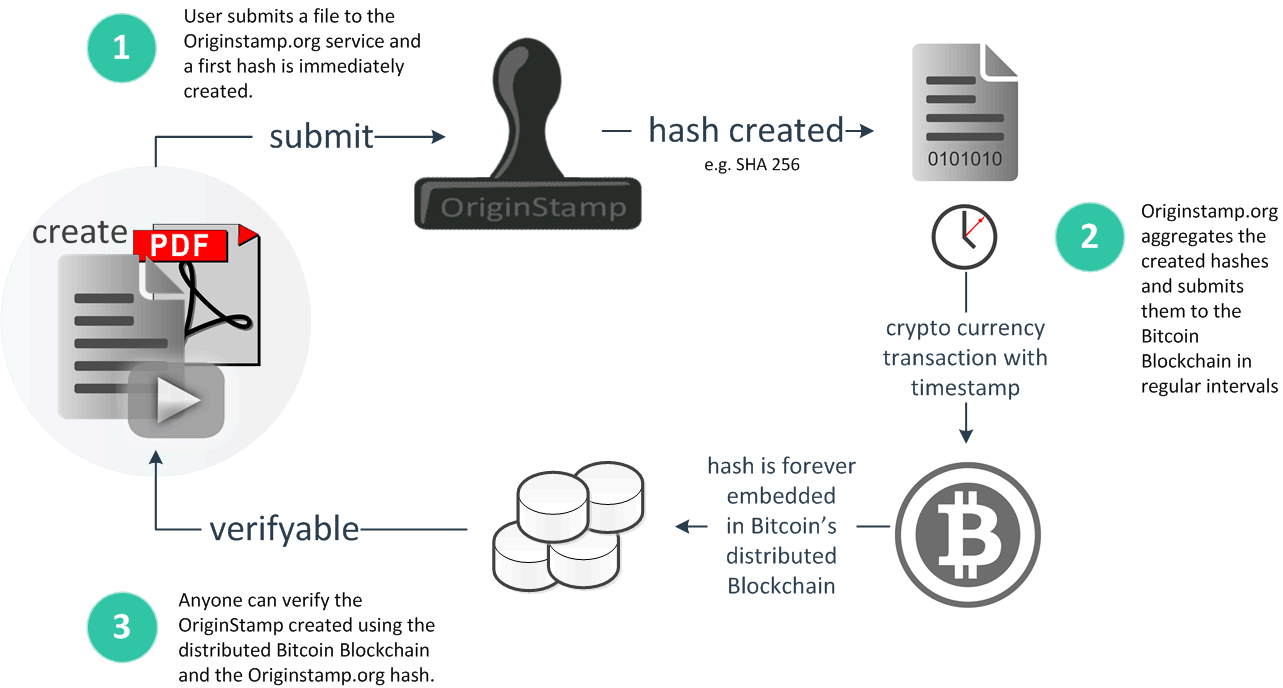
\includegraphics[scale=0.5]{sections/developement/originStamp_workflow.png}
\centering
\caption{OriginStamp}
\label{fig:originStamp}
\end{figure}
\newline La Figura \ref{fig:originStamp}, extreta de la documentació del propi servei, ens mostra el seu funcionament.\\
Tal i com indica l'anterior figura, \textit{OriginStamp} agrega \textit{hash} durant un lapse determinat de temps (24 hores). Un cop passat aquest lapse, afegeix els \textit{hash} que ha acumulat a la \textit{blockchain}, quedant ja per sempre registrats.\\
%\newline Com tot bon servei, ofereix una API amb la qual treballar i integrar els seus serveis al projecte.\\
\newline Continuant amb l'arquitectura general del projecte, aquesta funcionalitat s'ha encapsulat en un servei que permet la re-utilització d'aquest codi en qualsevol punt del projecte.\\
A nivell d'implementació, es tracta de fer crides \textit{HTTP/Post} a la API amb el \textit{hash} en qüestió.\\
\newline A més a més de la \textit{blockchain}, s'ha decidit fer ús d'un servei de segellat de temps (en anglès \textit{timestamping}) per a donar més força a la signatura del consentiment informat.\\
Aquest servei, oferit per FreeTSA\footnote{\url{https://freetsa.org}} permet crear peticions de timestamp (tsq) mitjançant \textit{OpenSSL}.\\
\newline La implementació és similar a la del servei anterior, el servei que encapsula la funcionalitat de \textit{timestamping} fa de pont entre el backend del projecte i el servei de \textit{FreeTSA}.
%A l'annex titulat ``\nameref{appendix:tsa}'' es pot veure la implementació sencera del servei que permet crear els segells de temps sobre els hash dels documents generats.\\
\newline Amb aquests dos serveis fent la mateixa funció, però en serveis que fan servir tecnologies diferents, aconseguim un sistema robust amb doble verificació de signatura, una per part de \textit{blockchain} i l'altre per part de la TSA.\\
Ambdós serveis, a més a més, disposen de mètodes de validació d'existència del \textit{hash}, un afegit amb un valor molt alt de cara el projecte.
\clearpage
\subsubsection{Refactor i millores}
Un cop acabat el desenvolupament global del projecte, s'han aplicat millores al projecte que cal esmentar.\\
Particularment la que fa referència a la creació dels documents.\\
\newline Fins ara, recordem que la creació de documents era responsabilitat del propi \textit{backend} quefeia ús de la llibreria de renderitzat \textit{Twig} i d'una llibreria externa per a la conversió de les plantilles en \textit{HTML} a pdf.\\
\newline Tot i les grans capacitats del tàndem que formen \textit{twig} i la llibreria \textit{wkhtmltopdf}, el punt flac d'aquest duo és la gran latència a l'hora de generar documents pdf.\\
\newline Per aquest motiu, aprofitant la incursió de l'us de serveis externs al projecte, s'ha decidit crear un petit servei,  en forma d'API Rest externa al \textit{backend} del projecte, que permeti la creació de documents de forma dinàmica a partir de plantilles bastant més riques que les emprades amb \textit{twig}, i sobre tot, amb una velocitat major.\\
\newline Als annexos ``\nameref{appendix:informed_consent}'' i ``\nameref{appendix:signature_receipt}'' es poden veure exemples dels dos documents generats amb aquest nou sistema.
    



